\documentclass{beamer}

\usepackage[italian]{babel}
\usepackage[utf8]{inputenc}
\usepackage[T1]{fontenc}
\usepackage{graphicx}
\usepackage{listings}
\usepackage{multicol}
\usepackage{mathtools}
\usepackage{color}
\usepackage[labelformat=empty]{caption}
\definecolor{brilliantrose}{rgb}{1.0, 0.33, 0.64}


\lstset{language=java,basicstyle=\tiny\ttfamily, columns=fullflexible,
keywordstyle=\color{red}\bfseries, commentstyle=\color{blue}, frame= single,}
\renewcommand{\lstlistingname}{Codice}


\usetheme{Frankfurt}
\setbeamercovered{dynamic}
\newcommand{\nologo}{\setbeamertemplate{logo}{}} % command to set the logo to nothing


\title{Testing of chosen Design Patterns with JUnit and Mockito}
\author{\textbf{{\large Niccolò Fabbri}}}
\author{\textbf{{\large Francesco Santoni}}}
\institute{Università degli Studi di Firenze\\ Corso di Laurea Triennale in Ingegneria Informatica}
\date{24 August 2016}
\logo{
\includegraphics[width=15mm]{logo-unifi-1}}
\begin{document}

\frame{\titlepage

 Relatore: Prof. Alessandro Fantechi \\
 Correlatore: Ing. Fabrizio Dini \\
 }
\nologo
\begin{section}{Introduction}
\begin{subsection}{Introduction}
\begin{frame}
\frametitle{Introduction}

In this paper we identify a collection of structural and behavioral design patterns: Class Adapter, Object Adapter, Proxy, Decorator, Composite, Observer, State, Visitor.

% ordine degli strutturali è individuato dalla "naturale" evoluzione in complessità della topologia% 
For each pattern we realize an implementation in Java and we develop a reasoned test suite based on a realistic fault model and on chosen coverage criteria.

We realize the tests through the \textit{JUnit} plug-in for Eclipse and the \textit{Mockito} framework. \textit{EclEmma} is used to provide a code coverage measure.
\end{frame}
\end{subsection}
\end{section}

\begin{section}{Design Patterns}
	\begin{subsection}{Design Patterns}
		\begin{frame}
			\frametitle{Class Adapter}
Adapts a pre-existent class to a new interface through inheritance. Through the new interface the old methods can be directly presented, modified, produce aggregated results or completely new functionality can be added.

\begin{figure}[!h]
	\centering
	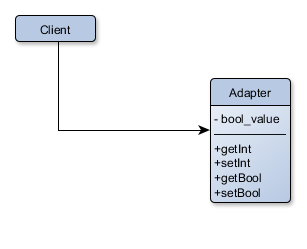
\includegraphics[width=0.7\textwidth]{./Adapter/Class/ClassDiagram.png}	
	\label{CAclassDiag}
\end{figure} 

		\end{frame}
	\end{subsection}
	
	
	\begin{subsection}{Design Patterns}
		\begin{frame}
			\frametitle{Class Adapter - Fault Model}
Given that the pattern focuses on allowing access to legacy methods through a new interface, failures are found in the following situations:  
\begin{itemize}
	\item the adapter did not inherit from the legacy class or the new interface
	\item the adapter cannot interact with the legacy methods 
\end{itemize}
\vspace{5mm}
The two sources of failure both depend on the inability of the Client to reach the Adaptee methods through the Adapter.  We reasoned that it is thus sufficient to test the ways in which the variable \textit{bool\_value} interacts and is modified by the methods.
			
		\end{frame}
	
	\end{subsection}
	
	\begin{subsection}{Design Patterns}
		\begin{frame}
			\frametitle{Class Adapter - Data Flow Graph}
	\begin{figure}[h]
		\centering
		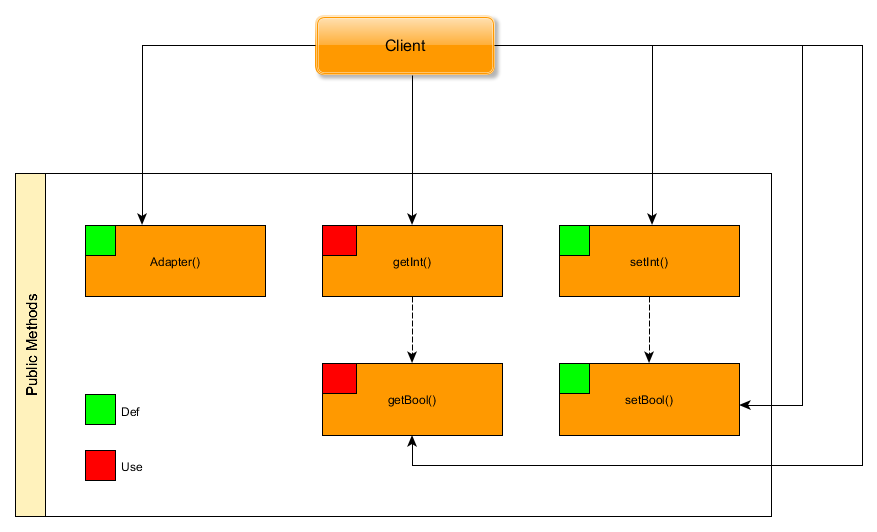
\includegraphics[width=0.7\textwidth]{./Adapter/Class/CallGraph.png}	
		\label{CAdataflow}
	\end{figure}
	
\vspace{5mm}
{\footnotesize 	We generated a test suite capable of testing all the \textit{all-uses} paths:
	\begin{itemize}
		\item Adapter() getInt() 
		\item Adapter() getBool() 
		\item Adapter() setInt() getInt() 
		\item Adapter() setInt() getBool() 
		\item Adapter() setBool() getInt()
		\newline
	\end{itemize}}

\end{frame}
\end{subsection}

	\begin{subsection}{Design Patterns}
		\begin{frame}
			\frametitle{Object Adapter}
Adapts a pre-existent class to a new interface through class composition. 

{\small Through the new interface the old methods can be directly presented, modified, produce aggregated results or completely new functionality can be added.}			

\begin{figure}[!h]
	\centering
	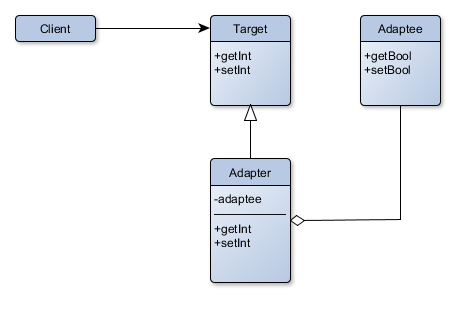
\includegraphics[width=0.7\textwidth]{./Adapter/Object/ClassDiagram.png}	
	\label{OAclassDiag}
\end{figure} 
			
		\end{frame}
	\end{subsection}

\begin{subsection}{Design Patterns}
\begin{frame}
	\frametitle{Object Adapter - Fault Model}
	
	Given that the pattern focuses on allowing access to legacy methods through a new interface, failures are found in the following situations:  
	\begin{itemize}
		\item the adapter did not inherit from the legacy class or the new interface
		\item the adapter cannot interact with the legacy methods 
		\item the instance contained in the adapter, which inherited the adaptee class, has overrode its methods in an unforeseen way
	\end{itemize}
\vspace{5mm}
	The sources of failure depend on the inability of the Client to reach the Adaptee methods through the Adapter or in the inability of the Adapter in foreseeing the possible ways in which the Adaptee methods can be overridden:  we reasoned that it is sufficient to test the ways in which the variable \textit{bool\_value} interacts and is modified by the methods, considering all the possible alternative implementations. 

\end{frame}
	\end{subsection}


\begin{subsection}{Design Patterns}
	\begin{frame}
		\frametitle{Object Adapter - Data Flow Graph}
		\begin{figure}[h]
			\centering
			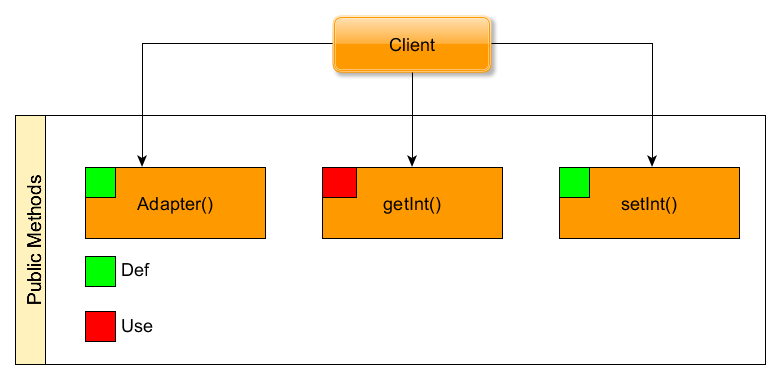
\includegraphics[width=0.75\textwidth]{./Adapter/Object/CallGraph.png}	
			\label{CAdataflow}
		\end{figure}
		We generated a test suite capable of testing all the \textit{all-uses} paths:
		\begin{itemize}
			\item Adapter() getInt() 
			\item Adapter() setInt() getInt() 
			
		\end{itemize}
		To these are also added the topology tests:
		\begin{itemize}
			\item Adapter( Adaptee ) getInt() 
			\item Adapter( AdapteeOpposite ) getInt()
		\end{itemize}	
		Of these the first, being already tested in the first suite, is not repeated.
		
			
		\end{frame}
	\end{subsection}



	\begin{subsection}{Design Patterns}
		\begin{frame}
			\frametitle{Proxy}
The Proxy pattern is constituted by a class  functioning as an interface to something else, usually a complex or heavy object.

{\small It is called by the client to access the real serving object behind the scenes, it either provides a cached result or transmits the request to the actual object.
}			
			
\begin{figure}[!h]
	\centering
	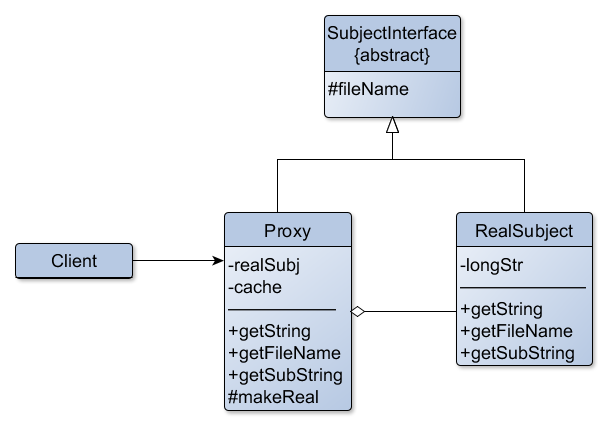
\includegraphics[width=0.7\textwidth]{./Proxy/ClassDiagram.png}
	\label{ProclassDiag}
\end{figure} 
			
		\end{frame}
	\end{subsection}


\begin{subsection}{Design Patterns}
	\begin{frame}
		\frametitle{Proxy - Fault Model}
		
		The pattern focuses on optimizing or controlling the access to the heavy subject. We have failures in the following situations:  
		\begin{itemize}
			\item the access to the RealSubject is impeded
			\item the cached copies provided by the Proxy differ from the actual source.
		\end{itemize}
		\vspace{5mm}
	The sources of failure depend on the inability of the Client to reach the RealSubject fields through the Proxy or in the inability of the Proxy of providing correct cached versions:  we reasoned that it is sufficient to test the ways in which the variable \textit{realSubj} interacts and is modified by the methods, by slight modification of the tests we can automatically verify the cached versions validity. 
		
	\end{frame}
\end{subsection}



\begin{subsection}{Design Patterns}
	\begin{frame}
		\frametitle{Proxy - Data Flow Graph}
		\begin{figure}[!h]
		\centering
		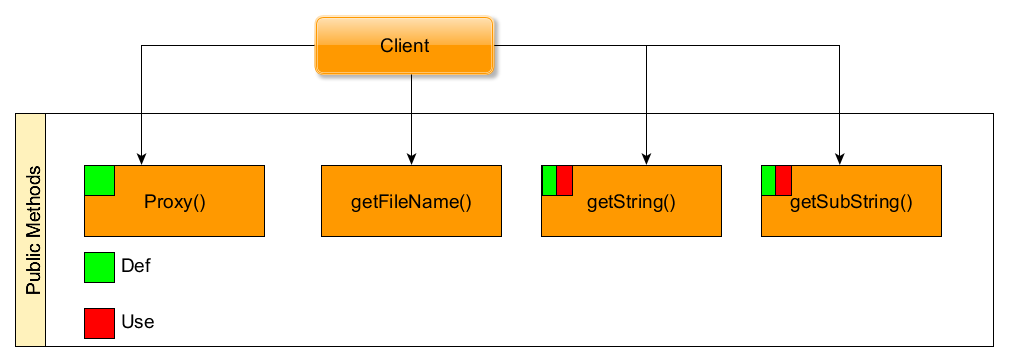
\includegraphics[width=0.8\textwidth]{./Proxy/CallGraph.png}
		
		\label{Prodataflow}
	\end{figure}
		{\footnotesize We generated a test suite capable of testing all the \textit{all-uses} paths:
		\begin{itemize}
			\item Proxy() getString() 
			\item Proxy() getString() getString()
			\item Proxy() getSubString()
			\item Proxy() getString() getSubString()
			\item Proxy() getSubString() getSubString()
			\item Proxy() getSubString() getString()			
		\end{itemize}
		}In particular  \textit{Proxy() getSubString() getSubString()} was altered to test the returned cached version after each method call. 		
	\end{frame}
\end{subsection}

\begin{subsection}{Design Patterns}
	\begin{frame}
		\frametitle{Decorator}
		The Decorator pattern allows behavior to be added to an individual object, either statically or dynamically, without affecting the behavior of other objects from the same class.

\begin{figure}[!h]
	\centering
	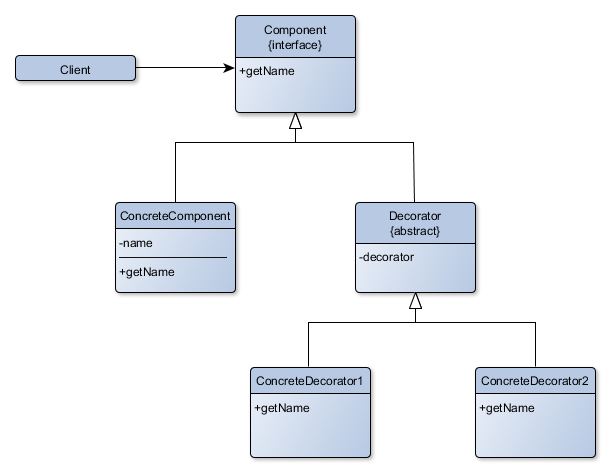
\includegraphics[width=0.7\textwidth]{./Decorator/ClassDiagram.png}	
	\label{DeclassDiag}
\end{figure} 
		
	\end{frame}
\end{subsection}

\begin{subsection}{Design Patterns}
	\begin{frame}
		\frametitle{Decorator - Fault Model}
		
		The pattern focuses on allowing an extension of functionality in objects. Grave errors are found in the following situations:  
		\begin{itemize}
			\item the call to the \textbf{operation (getName)} does not reach the Component or results in unexpected behavior
		\end{itemize}
		\vspace{5mm}
	The sources of failure depend on the presence of errors in the sequence of additive behavior to the \textit{operation (getName)}. We reasoned that to produce a satisfying test suite it is sufficient to test the correctness of the sequence of method calls in different hierarchies of classes.
		
	\end{frame}
\end{subsection}

\begin{subsection}{Design Patterns}
	\begin{frame}
		\frametitle{Decorator - Class Dependency Graph}
\begin{figure}[!h]
	\centering
	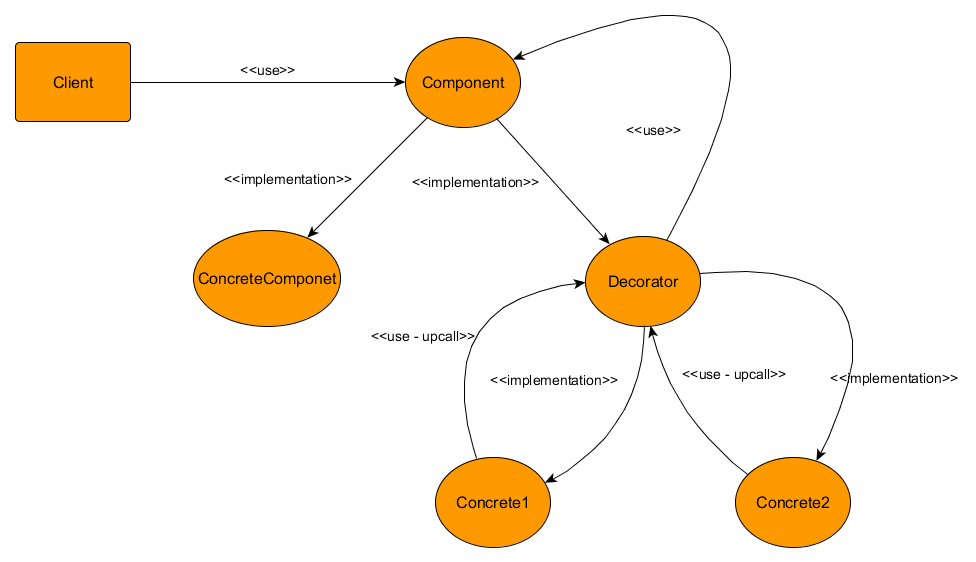
\includegraphics[width=0.8\textwidth]{./Decorator/ClassDepencyGraph.png}
	\label{Dedepengraph}
\end{figure}
{\footnotesize We decided to generate a test suite dependent on the \textit{all-edges} criterion.
We identified the 3 cases of:}
\begin{itemize}
	\item ConcreteComponent
	\item Decorator ConcreteComponent
	\item Decorator Decorator ConcreteComponent
	
\end{itemize}
{\footnotesize as representative of the entire set of possible hierarchies.
We then tested the \textit{getName()} method on the identified cases.} 		
	\end{frame}
\end{subsection}

\begin{subsection}{Design Patterns}
	\begin{frame}
		\frametitle{Composite}
The Composite pattern "composes" objects into tree structures to represent part-whole hierarchies. Implementing the composite pattern lets clients treat individual objects and compositions uniformly.

\begin{figure}[!h]
	\centering
	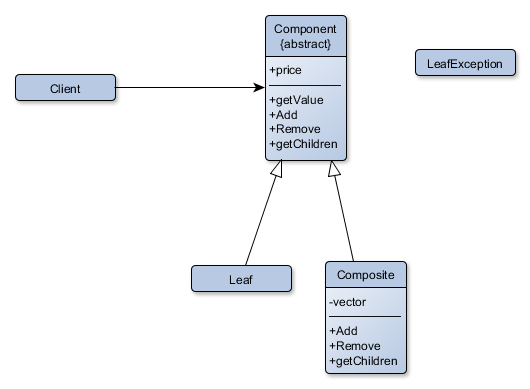
\includegraphics[width=0.7\textwidth]{./Composite/ClassDiagram.png}
	\label{CoclassDiag}
\end{figure}
		
	\end{frame}
\end{subsection}

\begin{subsection}{Design Patterns}
	\begin{frame}
		\frametitle{Composite - Fault Model}
		
The pattern focuses on treating uniformly individual and compound objects. Grave errors are found in the following situations:  
\begin{itemize}
	\item the common \textit{operation} works differently than expected
	\item the composite-specific methods produce unexpected effects when called on a Leaf object
\end{itemize}
		\vspace{5mm}
The sources of failure depend on the inability of the specific components (individual or composite parts) to be interacted in an uniform way. We reasoned that to produce a satisfying test suite we must test two different things: the way \textit{operation} works under the possible hierarchies at runtime and the way the different objects behave under calls from composite-specific methods.
		
	\end{frame}
\end{subsection}

\begin{subsection}{Design Patterns}
	\begin{frame}
		\frametitle{Composite - Data Flow Graph}

\begin{figure}[!h]
	\centering
	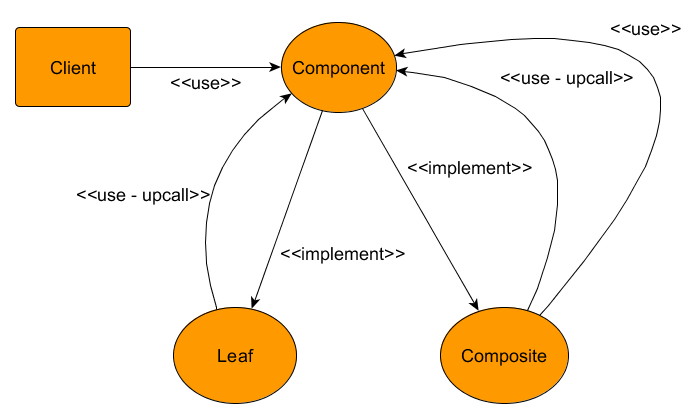
\includegraphics[width=0.8\textwidth]{./Composite/ClassDepencyGraph.png}	
	\label{Codepengraph}
\end{figure}
We generated a test suite capable of testing all the \textit{all-uses} paths:
\begin{itemize}
	\item Component() getChild()
	\item Component() getValue()
	\item Component() add() getChild()
	\item Component() add() getValue()
	\item Component() add() add() remove() getChild()
	\item Component() add() add() remove() getValue() 
\end{itemize} 		
	\end{frame}
\end{subsection}

\begin{subsection}{Design Patterns}
	\begin{frame}
		\frametitle{Composite - Class Dependency Graph}
		
		\begin{figure}[!h]
			\centering
			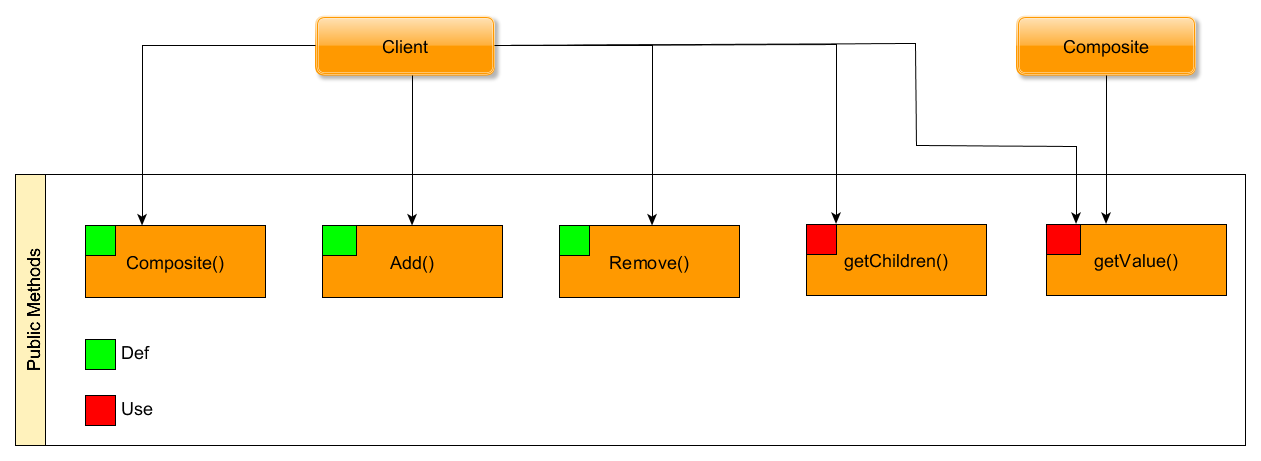
\includegraphics[width=0.8\textwidth]{./Composite/CallGraph.png}
			
			\label{Codataflow}
		\end{figure}
We identified the 3 cases of:
\begin{itemize}
	\item single Leaf
	\item Composite containing Leaf
	\item Composite containing Composite
\end{itemize}
as representative of the entire set of possible hierarchies.

We then tested all the composite-specific methods (add, remove, getChild) on the identified cases.	
	\end{frame}
\end{subsection}

\begin{subsection}{Design Patterns}
	\begin{frame}
		\frametitle{Observer}
		In the Observer pattern an object, called the subject, maintains a list of its dependents, called observers, and notifies them automatically of any state changes, usually by calling one of their methods.
		
\begin{figure}[!h]
	\centering
	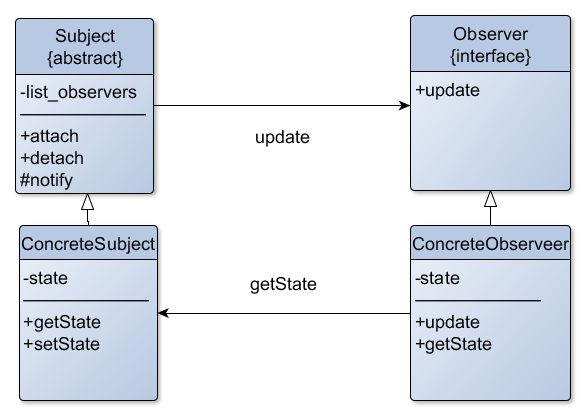
\includegraphics[width=0.7\textwidth]{./Observer/ClassDiagram.png}
	\label{ObclassDiag}
\end{figure}
		
	\end{frame}
\end{subsection}

\begin{subsection}{Design Patterns}
	\begin{frame}
		\frametitle{Observer - Fault Model}
The pattern focuses on maintaining updated objects that expressed the interest in a specific subject. Failures are found in the following situations:  
\begin{itemize}
	\item \textit{attach} and \textit{detach} do not produce the expected results.
	\item after a change of the subject state the following observers are not \textit{notified}.
	\item the observer after being notified does not execute correctly the \textit{update} method.
\end{itemize}
		\vspace{5mm}
		The sources of failure depend on the presence of problems that impede the correct functioning of the inter-class methods and, in the lesser part, by the inability of the observer to correctly update. We considered the correct modification on the subject internal \textit{state} as not important for our pattern.  We reasoned that to produce a satisfying test suite we must test the way \textit{list\_observers} is modified after an inter-class method invocation and the way the \textit{state} of the observer is modified after a notification.
		
	\end{frame}
\end{subsection}

\begin{subsection}{Design Patterns}
	\begin{frame}
		\frametitle{Observer - Data Flow Graph: field \textit{list\_observer}}
		
		We decided to test the interaction between the variable and the methods
		following the all-uses criterion, we deemed the all-def criterion excessively restrictive to test this pattern.
\begin{figure}[!h]
	\centering
	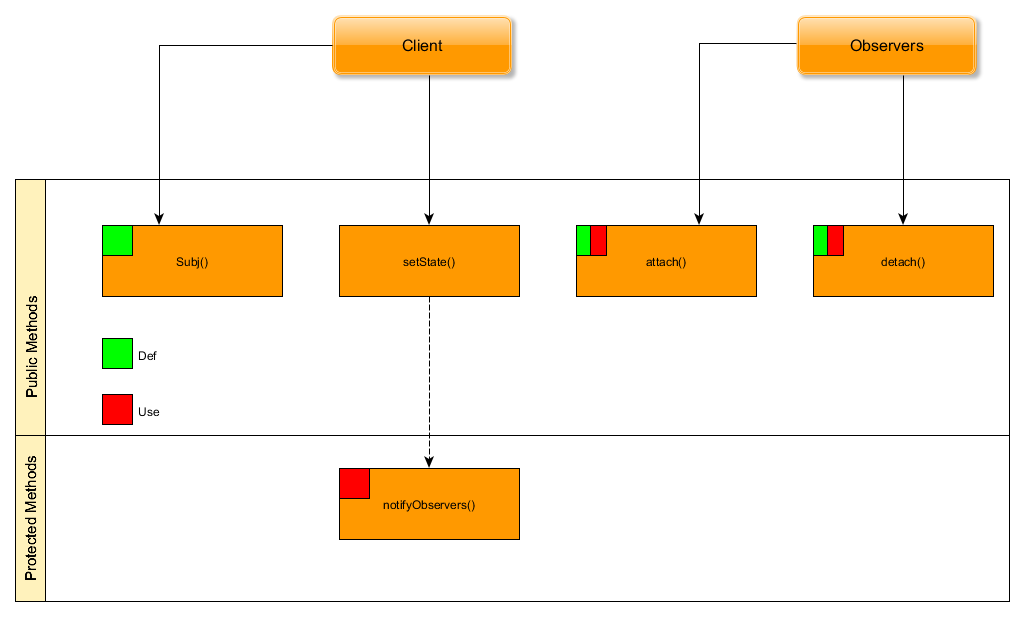
\includegraphics[width=0.8\textwidth]{./Observer/CallGraph.png}
	\label{Obdataflow1}
\end{figure} 		
	\end{frame}
\end{subsection}

\begin{subsection}{Design Patterns}
	\begin{frame}
		\frametitle{Observer - Data Flow Graph: field \textit{state}}
		
		\begin{figure}[!h]
			\centering
			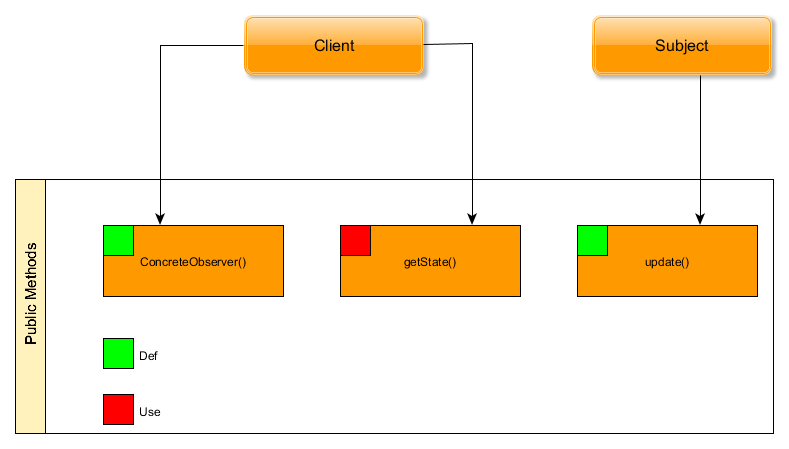
\includegraphics[width=0.8\textwidth]{./Observer/CallGraph_State.png}
			\caption{Data Flow Graph: \textit{state}}
			\label{Obdataflow2}
		\end{figure}
		
We generated a test suite capable of testing all the \textit{all-uses} paths:
\begin{itemize}
	\item ConcreteObserver() getState()
	\item ConcreteObserver() update() getState()
	
\end{itemize}
In both type of tests, since the tested class's methods (ConcreteSubject and ConcreteObserver) interacted with external classes (Observer and Subject) we  differentiated between Unit and Integration tests.		
	\end{frame}
\end{subsection}

\begin{subsection}{Design Patterns}
	\begin{frame}
		\frametitle{Observer - Fault Model}
		The pattern focuses on maintaining updated objects that expressed the interest in a specific subject. Failures are found in the following situations:  
		\begin{itemize}
			\item \textit{attach} and \textit{detach} do not produce the expected results.
			\item after a change of the subject state the following observers are not \textit{notified}.
			\item the observer after being notified does not execute correctly the \textit{update} method.
		\end{itemize}
		\vspace{5mm}
		The sources of failure depend on the presence of problems that impede the correct functioning of the inter-class methods and, in the lesser part, by the inability of the observer to correctly update. We considered the correct modification on the subject internal \textit{state} as not important for our pattern.  We reasoned that to produce a satisfying test suite we must test the way \textit{list\_observers} is modified after an inter-class method invocation and the way the \textit{state} of the observer is modified after a notification.
		
	\end{frame}
\end{subsection}

\begin{subsection}{Design Patterns}
	\begin{frame}
		\frametitle{State}
		The State pattern implements a state machine by implementing each individual state as a derived class of the state pattern interface, and implementing state transitions by invoking methods defined by the pattern's superclass.
\begin{figure}[!h]
	\centering
	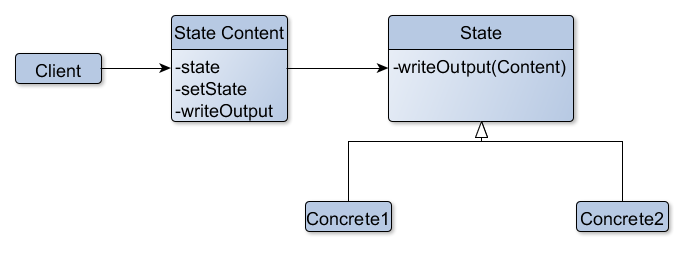
\includegraphics[width=0.7\textwidth]{./State/ClassDiagram.png}
	\label{SclassDiag}
\end{figure}
		
	\end{frame}
\end{subsection}

\begin{subsection}{Design Patterns}
	\begin{frame}
		\frametitle{State - Fault Model}
		The pattern focuses on delegating the actual methods implementation to internal state classes. Grave errors are found in the following situations:  
		\begin{itemize}
			\item internal state changes in an erroneous manner. 
			\item the internal state methods produce unexpected side effects or results.
			\item (with less importance) the internal classes' inner state changes in an erroneous manner.
		\end{itemize}
		\vspace{5mm}
		The sources of failure depend on the presence of problems that impede the correct functioning of the inter-class methods and, in the lesser part, by the inability of the observer to correctly update. We considered the correct modification on the subject internal \textit{state} as not important for our pattern.  We reasoned that to produce a satisfying test suite we must test the way \textit{list\_observers} is modified after an inter-class method invocation and the way the \textit{state} of the observer is modified after a notification.
		
	\end{frame}
\end{subsection}

\begin{subsection}{Design Patterns}
	\begin{frame}
		\frametitle{State - Data Flow Graph}
\begin{figure}[!h]
	\centering
	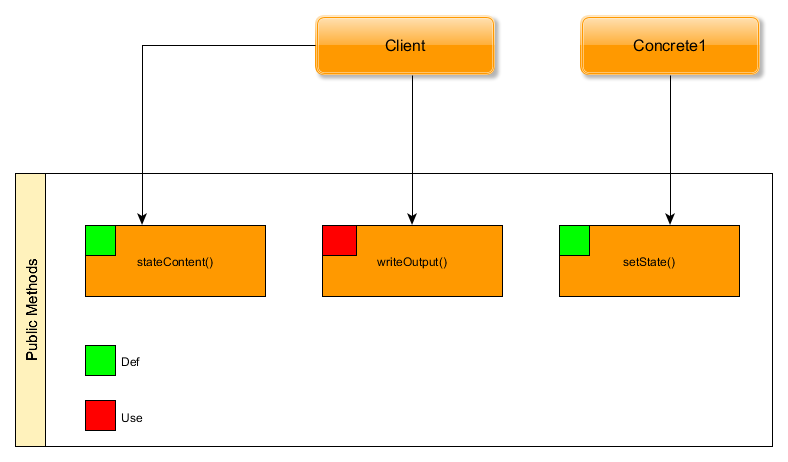
\includegraphics[width=0.8\textwidth]{./State/CallGraph.png}
	\label{Sdataflow}
\end{figure}

We generated a test suite capable of testing all the \textit{all-uses} paths:
\begin{itemize}
	\item StateContext() writeOutput() 
	\item StateContext() setState() writeOutput()
	\item StateContext() writeOutput() writeOutput()
\end{itemize}

The last test case is actually used to test the correctness of the way ConcreteStates update the field and does not cover a particular D-U path.
	
	\end{frame}
\end{subsection}

\begin{subsection}{Design Patterns}
	\begin{frame}
		\frametitle{Visitor}
The Visitor pattern is a way of separating an algorithm from an object structure on which it operates. {\footnotesize The pattern allows one to add new virtual functions to a family of classes without modifying the classes themselves: the visitor class implements all of the appropriate specializations of the virtual function. The visitor takes the instance reference as input, and implements the goal through double dispatch.}
		
\begin{figure}[!h]
	\centering
	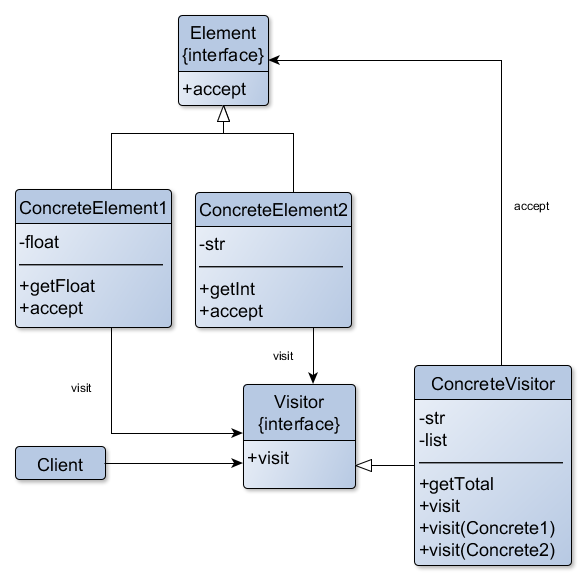
\includegraphics[width=0.7\textwidth]{./Visitor/ClassDiagram.png}
	\label{ViclassDiag}
\end{figure}
		
	\end{frame}
\end{subsection}

\begin{subsection}{Design Patterns}
	\begin{frame}
		\frametitle{Visitor - Fault Model}
The pattern focuses on treating uniformly objects of different types while operating on them with different specializations of the same function. A failure is produced by the following situation:  
\begin{itemize}
	\item the wrong \textit{visit()} is applied to an Element
\end{itemize}
		\vspace{5mm}
The sources of failure depend on the inability of the Visitor to identify the specialized implementation to execute. This depends mainly on the type of Element we are working with. We thus reasoned that to produce a satisfying test suite we must test the way \textit{visit} works when applied to all possible hierarchies of Element types.
		
	\end{frame}
\end{subsection}

\begin{subsection}{Design Patterns}
	\begin{frame}
		\frametitle{Visitor - Class Dependency Graph}
		
\begin{figure}[!h]
	\centering
	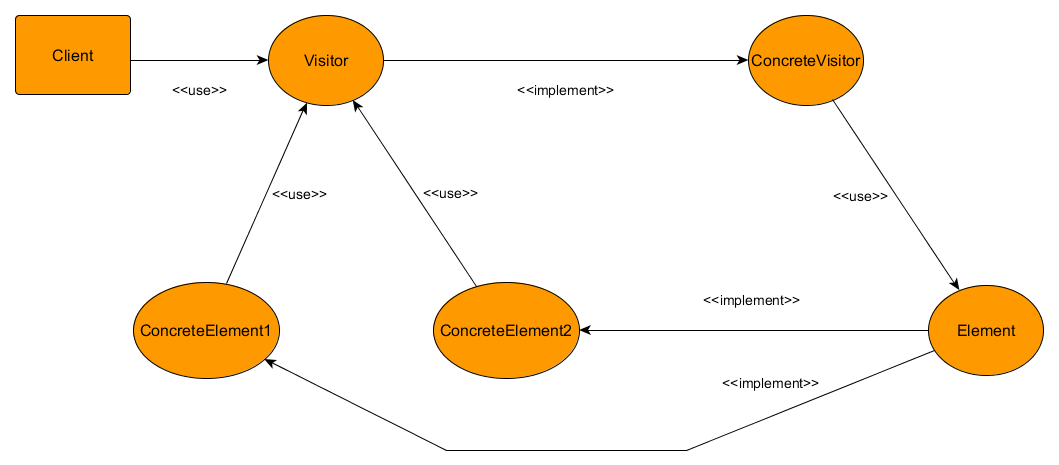
\includegraphics[width=0.8\textwidth]{./Visitor/ClassDependencyGraph.png}
	\label{Videpengraph}
\end{figure}
We identified the 2 cases of:
\begin{itemize}
	\item Visitor ConcreteVisitor Element ConcreteElement2 Visitor
	\item Visitor ConcreteVisitor Element ConcreteElement1 Visitor	
\end{itemize}
as representative of the entire set of possible hierarchies.
	\end{frame}
\end{subsection}





	
\end{section}


\end{document}